%% This file was auto-generated by IPython.
%% Conversion from the original notebook file:
%% pca.ipynb
%%
\documentclass[11pt,english,fleqn]{article}

%% This is the automatic preamble used by IPython.  Note that it does *not*
%% include a documentclass declaration, that is added at runtime to the overall
%% document.

\usepackage{amsmath}
\usepackage{amssymb}
\usepackage{graphicx}
\usepackage{ucs}
\usepackage[utf8x]{inputenc}

% needed for markdown enumerations to work
\usepackage{enumerate}

% Slightly bigger margins than the latex defaults
\usepackage{geometry}
\geometry{verbose,tmargin=3cm,bmargin=3cm,lmargin=2.5cm,rmargin=2.5cm}

% Define a few colors for use in code, links and cell shading
\usepackage{color}
\definecolor{orange}{cmyk}{0,0.4,0.8,0.2}
\definecolor{darkorange}{rgb}{.71,0.21,0.01}
\definecolor{darkgreen}{rgb}{.12,.54,.11}
\definecolor{myteal}{rgb}{.26, .44, .56}
\definecolor{gray}{gray}{0.45}
\definecolor{lightgray}{gray}{.95}
\definecolor{mediumgray}{gray}{.8}
\definecolor{inputbackground}{rgb}{.95, .95, .85}
\definecolor{outputbackground}{rgb}{.95, .95, .95}
\definecolor{traceback}{rgb}{1, .95, .95}

% Framed environments for code cells (inputs, outputs, errors, ...).  The
% various uses of \unskip (or not) at the end were fine-tuned by hand, so don't
% randomly change them unless you're sure of the effect it will have.
\usepackage{framed}

% remove extraneous vertical space in boxes
\setlength\fboxsep{0pt}

% codecell is the whole input+output set of blocks that a Code cell can
% generate.

% TODO: unfortunately, it seems that using a framed codecell environment breaks
% the ability of the frames inside of it to be broken across pages.  This
% causes at least the problem of having lots of empty space at the bottom of
% pages as new frames are moved to the next page, and if a single frame is too
% long to fit on a page, will completely stop latex from compiling the
% document.  So unless we figure out a solution to this, we'll have to instead
% leave the codecell env. as empty.  I'm keeping the original codecell
% definition here (a thin vertical bar) for reference, in case we find a
% solution to the page break issue.

%% \newenvironment{codecell}{%
%%     \def\FrameCommand{\color{mediumgray} \vrule width 1pt \hspace{5pt}}%
%%    \MakeFramed{\vspace{-0.5em}}}
%%  {\unskip\endMakeFramed}

% For now, make this a no-op...
\newenvironment{codecell}{}

 \newenvironment{codeinput}{%
   \def\FrameCommand{\colorbox{inputbackground}}%
   \MakeFramed{\advance\hsize-\width \FrameRestore}}
 {\unskip\endMakeFramed}

\newenvironment{codeoutput}{%
   \def\FrameCommand{\colorbox{outputbackground}}%
   \vspace{-1.4em}
   \MakeFramed{\advance\hsize-\width \FrameRestore}}
 {\unskip\medskip\endMakeFramed}

\newenvironment{traceback}{%
   \def\FrameCommand{\colorbox{traceback}}%
   \MakeFramed{\advance\hsize-\width \FrameRestore}}
 {\endMakeFramed}

% Use and configure listings package for nicely formatted code
\usepackage{listingsutf8}
\lstset{
  language=python,
  inputencoding=utf8x,
  extendedchars=\true,
  aboveskip=\smallskipamount,
  belowskip=\smallskipamount,
  xleftmargin=2mm,
  breaklines=true,
  basicstyle=\small \ttfamily,
  showstringspaces=false,
  keywordstyle=\color{blue}\bfseries,
  commentstyle=\color{myteal},
  stringstyle=\color{darkgreen},
  identifierstyle=\color{darkorange},
  columns=fullflexible,  % tighter character kerning, like verb
}

% The hyperref package gives us a pdf with properly built
% internal navigation ('pdf bookmarks' for the table of contents,
% internal cross-reference links, web links for URLs, etc.)
\usepackage{hyperref}
\hypersetup{
  breaklinks=true,  % so long urls are correctly broken across lines
  colorlinks=true,
  urlcolor=blue,
  linkcolor=darkorange,
  citecolor=darkgreen,
  }

% hardcode size of all verbatim environments to be a bit smaller
\makeatletter 
\g@addto@macro\@verbatim\small\topsep=0.5em\partopsep=0pt
\makeatother 

% Prevent overflowing lines due to urls and other hard-to-break entities.
\sloppy

\setlength{\mathindent}{0pt}
\setlength{\parindent}{0pt}
\setlength{\parskip}{8pt}
\begin{document}

Temel Bileşen Analizi (Principal Component Analysis -PCA-)

PCA yontemi boyut azaltan yontemlerden biridir, takip edilmeden
(unsupervised) isleyebilir. Ana fikir veri noktalarinin izdusumunun
yapilacagi yonler bulmaktir ki bu yonler baglaminda (izdusum sonrasi)
noktalarin arasindaki varyans (variance) en fazla olsun, yani noktalar
en ``yaygin'' sekilde bulunsunlar. Boylece birbirinden daha uzaklasan
noktalarin mesela daha rahat kumelenebilecegini umabiliriz. Yani bir
diger amac hangi degiskenlerin varyansinin daha fazla olmasinin
gorulmesi uzerine, o degiskenlerin daha onemli olabileceginin
anlasilmasi. Ornek olarak alttaki grafige bakalim,

\begin{codecell}
\begin{codeinput}
\begin{lstlisting}
from pandas import *
data = read_csv("testSet.txt",sep="\t",header=None)
data[:10]
\end{lstlisting}
\end{codeinput}
\begin{codeoutput}
\begin{verbatim}
           0          1
0  10.235186  11.321997
1  10.122339  11.810993
2   9.190236   8.904943
3   9.306371   9.847394
4   8.330131   8.340352
5  10.152785  10.123532
6  10.408540  10.821986
7   9.003615  10.039206
8   9.534872  10.096991
9   9.498181  10.825446
\end{verbatim}
\end{codeoutput}
\end{codecell}
\begin{codecell}
\begin{codeinput}
\begin{lstlisting}
scatter(data.ix[:,0],data.ix[:,1])
plot(data.ix[1,0],data.ix[1,1],'rd')
plot(data.ix[4,0],data.ix[4,1],'rd')
\end{lstlisting}
\end{codeinput}
\begin{codeoutput}
\begin{verbatim}
[<matplotlib.lines.Line2D at 0xb52880c>]
\end{verbatim}
\begin{center}
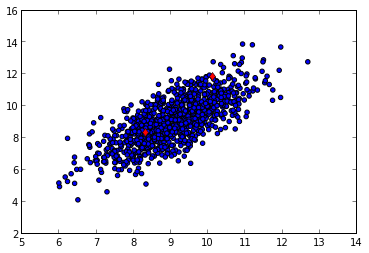
\includegraphics[width=0.7\textwidth]{pca_files/pca_fig_00.png}
\par
\end{center}
\end{codeoutput}
\end{codecell}
PCA ile yapmaya calistigimiz oyle bir yon bulmak ki, $x$ veri
noktalarinin tamaminin o yone izdusumu yapilinca sonuc olacak,
``izdusumu yapilmis'' $z$'nin varyansi en buyuk olsun. Bu bir
maksimizasyon problemidir. Fakat ondan once $x$ nedir, $z$ nedir bunlara
yakindan bakalim.

Veri $x$ ile tum veri noktalari kastedilir, fakat PCA probleminde
genellikle bir ``vektorun digeri uzerine'' yapilan izdusumu, ``daha
optimal bir $w$ yonu bulma'', ve ``o yone dogru izdusum yapmak''
kelimeleri kullanilir. Demek ki veri noktalarini bir vektor olarak
gormeliyiz. Eger ustte kirmizi ile isaretlenen iki noktayi alirsak (bu
noktalar verideki 1. ve 4. siradaki noktalar),

\begin{codecell}
\begin{codeinput}
\begin{lstlisting}
img=imread("proj1.png")
plt.imshow(img)

\end{lstlisting}
\end{codeinput}
\begin{codeoutput}
\begin{verbatim}
<matplotlib.image.AxesImage at 0xa9e5e2c>
\end{verbatim}
\begin{center}
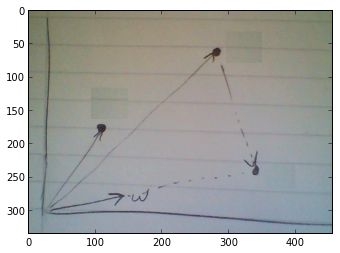
\includegraphics[width=0.7\textwidth]{pca_files/pca_fig_01.png}
\par
\end{center}
\end{codeoutput}
\end{codecell}
gibi bir goruntuden bahsediyoruz. Hayali bir $w$ kullandik, ve
noktalardan biri veri noktasi, $w$ uzerine izdusum yapilarak yeni bir
vektoru / noktayi ortaya cikartiyor. Genel olarak ifade edersek, bir
nokta icin
\[z = w^T x\]
Yapmaya calistigimiz varyansi maksimize etmek demistik. Ozel bir izdusum
yonunu referans alirsak, en buyuk $Var(z_1)$'i bulacagiz. Not: Bunu
soyler soylemez $x$'i ve $z$'yi rasgele degiskenler olarak gordugumuzu
belirtmis oluyoruz. Ardi ardina alet cantasindan temsili numaralari
kullaniyoruz - $x$'i bir yandan vektor yapiyoruz, bir yandan bir
dagilimdan gelen zar atisi gibi goruyoruz, problemi cozmemize ne yardim
edecekse onu surekli devreye sokuyoruz. Devam edelim, rasgele degisken
deyince, demek ki $x,z$ dagilimlardan gelecektir, bu dagilimlarin cok
boyutlu normal (multivariate normal) oldugunu kabul edebiliriz. Peki
eger $x$, $N(\mu,\Sigma)$ gibi cok boyutlu normal dagilimdan geliyorsa,
ki $\mu$ ortalama ve $\Sigma$ kovaryanstir, $w^Tx$ nedir?

Bu yeni ``seyin'' beklentisi ve varyansina bakalim,
\[ E[w^Tx] = w^T E[x] = w^T \mu \]\[ Var(w^Tx)  = w^T Var(x) w = w^T \Sigma w\]
Ustteki sonuclarin boyutlarina dikkat: $w^T \mu$ durumunda
$1 \times N \cdot N \times 1 = 1 \times 1$ , $w^T \Sigma w$ durumunda
ise $1 \times N \cdot N \times N \cdot N \times 1 = 1 \times 1$. Iki
durumda da tek boyutlu skalar degerler elde ettik. Demek ki $w^T$ ile
carpim sonrasi bir $N(w^T\mu,w^T\Sigma w)$ dagilimi elde ederiz ve bu
dagilim bir tek boyutlu bir dagilimdir. Yani $w$ yonundeki izdusum bize
tek boyutlu bir Gaussian dagilimini verecektir. Bu sonuc aslinda cok
sasirtici olmasa gerek, tum veri noktalarini alip, baslangici orijin
noktasinda olan vektorlere cevirip ayni yone isaret edecek sekilde
duzenliyoruz, bu vektorleri tekrar nokta olarak dusunursek, tabii ki
ayni yonu gosteriyorlar, bilahere ayni cizgi uzerindeki noktalara
donusuyorlar. Ayni cizgi uzerinde olmak ne demek? Tek boyuta inmis olmak
demek.

Bastaki amacimiza donersek, $Var(z_1)$'i maksimize etmek ayni anda
$Var(w_1^T\Sigma w_1)$'i maksimize etmek demektir.

Ufak bir sorun $w_1^T\Sigma w_1$'i surekli daha buyuk $w_1$'lerle sonsuz
kadar buyutebilirsiniz. Bize ek bir kisitlama sarti daha lazim, bu sart
$||w|| = 1$ olabilir, yani $w$'nin norm'u 1'den daha buyuk olmasin.
Boylece optimizasyon $w$'nin buyuklugu uzerinde taklalar atmayacak,
sadece yon bulmak ile ilgilenecek, iyi, zaten biz $w$'nin yonu ile
ilgileniyoruz. Aradigimiz ifadeyi yazalim, ve ek siniri Lagrange ifadesi
olarak ekleyelim, ve yeni bir $L$ ortaya cikartalim,
\[ L(w_1,\lambda) =  w_1^T \Sigma w_1  - \lambda(w_1^T w_1 - 1) \]
Niye eksiden sonraki terim o sekilde eklendi? O terim oyle sekilde
secildi ki, $\partial L / \partial \lambda = 0$ alininca $w_1^Tw_1 = 1$
geri gelsin / ortaya ciksin {[}2, sf 340{]}, bu Lagrange'in dahice
bulusu. Bunu kontrol edebilirsiniz, $\lambda$ 'ya gore turev alirken
$w_1$ sabit olarak yokolur, parantez icindeki ifadeler kalir ve sifira
esitlenince orijinal kisitlama ifadesi geri gelir. Simdi
\[ \max\limits_{w_1} L(w_1,\lambda) \]
Turevi $w_1$'e gore alirsak, ve sifira esitlersek,
\[ 2w_1 \Sigma - 2 \lambda w_1 = 0 \]\[ 2w_1 \Sigma = 2 \lambda w_1 \]\[ \Sigma w_1  = \lambda w_1 \]
Ustteki ifade ozdeger, ozvektor ana formulune benzemiyor mu? Evet. Eger
$w_1$, $\Sigma$'nin ozvektoru ise ve esitligin sagindaki $\lambda$ ona
tekabul eden ozdeger ise, bu esitlik dogru olacaktir.

Peki hangi ozdeger / ozvektor maksimal degeri verir? Unutmayalim,
maksimize etmeye calistigimiz sey $w_1^T \Sigma w_1$ idi

Eger $\Sigma w_1 = \lambda w_1$ yerine koyarsak
\[ w_1^T \lambda w_1 =  \lambda w_1^T  w_1 = \lambda \]
Cunku $w_1^T w$'nin 1 olacagi sartini koymustuk. Neyse, maksimize etmeye
calistigimiz deger $\lambda$ cikti, o zaman en buyuk $\lambda$
kullanirsak, en maksimal varyansi elde ederiz, bu da en buyuk ozdegerin
ta kendisidir.

Demek ki izdusum yapilacak ``yon'' kovaryans $\Sigma$'nin en buyuk
ozdegerine tekabul eden ozvektor olarak secilirse, temel bilesenlerden
en onemlisini hemen bulmus olacagiz.

Cebirin geri kalani $w_2$,$w_3$ icin devam eder, bu turetmenin
detaylarini {[}1{]} ve {[}2{]} gibi kaynaklarda bulabilirsiniz. Fakat
ulasilan sonuc en bilesenlerin onem sirasinin aynen ozdegerlerin
buyukluk sirasina tekabul ediyor olmasi.

Ornek
Simdi tum bunlari bir ornek uzerinde gorelim. Iki boyutlu ornek veriyi
ustte yuklemistik. Simdi veriyi ``sifirda ortalayacagiz'' yani her kolon
icin o kolonun ortalama degerini tum kolondan cikartacagiz. PCA ile
islem yaparken tum degerlerin sifir merkezli olmasi gerekiyor.

Daha sonra ozdegerlerini, vektorlerini hesaplayabilmek icin verinin
kovaryansini hesaplayacagiz.

\begin{codecell}
\begin{codeinput}
\begin{lstlisting}
means = mean(data, axis=0)
meanless_data = data - means
cov_mat = cov(meanless_data, rowvar=0)
eigs,eigv = linalg.eig(mat(cov_mat))
eig_ind = argsort(eigs)
eig_ind

\end{lstlisting}
\end{codeinput}
\begin{codeoutput}
\begin{verbatim}
array([0, 1])
\end{verbatim}
\end{codeoutput}
\end{codecell}
Ustteki sonuc sort sonrasi elde edilen indis degerleri, sort en kucukten
en buyuge dogru dizimi yapmistir, en buyuk ozdegerin indisi en sondadir.
Raslantisal bir sekilde en buyuk olan deger en sagda cikti ama tersi de
olabilirdi, neyse, bu ozdeger, vektorleri ekrana basalim,

\begin{codecell}
\begin{codeinput}
\begin{lstlisting}
print eigs[1],eigv[:,1].T
print eigs[0],eigv[:,0].T

\end{lstlisting}
\end{codeinput}
\begin{codeoutput}
\begin{verbatim}
2.89713495618 [[-0.52045195 -0.85389096]]
0.366513708669 [[-0.85389096  0.52045195]]
\end{verbatim}
\end{codeoutput}
\end{codecell}
En buyuk olan yonu quiver komutunu kullanarak orijinal veri seti
uzerinde gosterelim,

\begin{codecell}
\begin{codeinput}
\begin{lstlisting}
scatter(data.ix[:,0],data.ix[:,1]) 
quiver(9,9,eigv[1,1],eigv[0,1],scale=10,color='r') # merkez 9,9, kabaca secildi

\end{lstlisting}
\end{codeinput}
\begin{codeoutput}
\begin{verbatim}
<matplotlib.quiver.Quiver at 0xbb6254c>
\end{verbatim}
\begin{center}
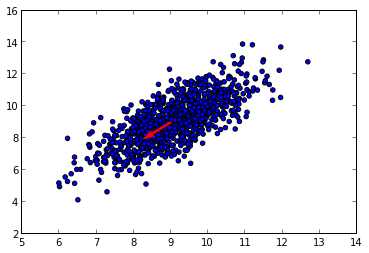
\includegraphics[width=0.7\textwidth]{pca_files/pca_fig_02.png}
\par
\end{center}
\end{codeoutput}
\end{codecell}
Goruldugu gibi bu yon hakikaten dagilimin, veri noktalarinin en cok
yayilmis oldugu yon. Demek ki PCA yontemi dogru sonucu buldu. Her iki
yonu de cizersek,

\begin{codecell}
\begin{codeinput}
\begin{lstlisting}
scatter(data.ix[:,0],data.ix[:,1]) 
quiver(9,9,eigv[1,0],eigv[0,0],scale=10,color='r') 
quiver(9,9,eigv[1,1],eigv[0,1],scale=10,color='r')

\end{lstlisting}
\end{codeinput}
\begin{codeoutput}
\begin{verbatim}
<matplotlib.quiver.Quiver at 0xc194c6c>
\end{verbatim}
\begin{center}
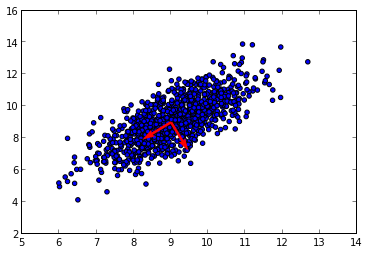
\includegraphics[width=0.7\textwidth]{pca_files/pca_fig_03.png}
\par
\end{center}
\end{codeoutput}
\end{codecell}
Bu ikinci yon birinciye dik olmaliydi, ve o da bulundu. Aslinda iki
boyut olunca baska secenek kalmiyor, 1. yon sonrasi ikincisi baska bir
sey olamazdi, fakat cok daha yuksek boyutlarda en cok yayilimin oldugu
ikinci yon de dogru sekilde geri getirilecekti.

{[}1{]} Alpaydin, E., Introduction to Machine Learning, 2nd Edition

{[}2{]} Strang, G., Linear Algebra and Its Applications, 4th Edition

{[}3{]}
http://www.stat.columbia.edu/\ensuremath{\sim}fwood/Teaching/w4315/Spring2010/PCA/slides.pdf

\end{document}
